\documentclass{article}

\def\ParSkip{} 
% Packages
\usepackage{amssymb,amsmath,amsthm,bbm}
\usepackage{verbatim,float,url,dsfont}
\usepackage{graphicx,subfigure,psfrag}
\usepackage{algorithm,algorithmic}
\usepackage{mathtools,enumitem}
\usepackage{multirow}
\usepackage{ragged2e}
\usepackage{xr-hyper}
\usepackage{array}

\usepackage[colorlinks=true,citecolor=blue,urlcolor=blue,linkcolor=blue]{hyperref}
\usepackage[margin=1in]{geometry}
\usepackage[round]{natbib}

\usepackage[utf8]{inputenc} % allow utf-8 input
\usepackage[T1]{fontenc}    % use 8-bit T1 fonts
\usepackage{booktabs}       % professional-quality tables
\usepackage{nicefrac}         % compact symbols for 1/2, etc.
\usepackage{microtype}      % microtypography

\ifdefined\TimesFont 
\usepackage{times} % use times font
\fi

\ifdefined\ParSkip 
\usepackage{parskip} % use par skip
\fi

% Theorems and such
\newtheorem{theorem}{Theorem}
\newtheorem{lemma}{Lemma}
\newtheorem{corollary}{Corollary}
\newtheorem{proposition}{Proposition}
\theoremstyle{definition}
\newtheorem{remark}{Remark}
\newtheorem{definition}{Definition}

% Assumption
\newtheorem*{assumption*}{\assumptionnumber}
\providecommand{\assumptionnumber}{}
\makeatletter
\newenvironment{assumption}[2]{
  \renewcommand{\assumptionnumber}{Assumption #1#2}
  \begin{assumption*}
  \protected@edef\@currentlabel{#1#2}}
{\end{assumption*}}
\makeatother

% Widebar
\makeatletter
\newcommand*\rel@kern[1]{\kern#1\dimexpr\macc@kerna}
\newcommand*\widebar[1]{%
  \begingroup
  \def\mathaccent##1##2{%
    \rel@kern{0.8}%
    \overline{\rel@kern{-0.8}\macc@nucleus\rel@kern{0.2}}%
    \rel@kern{-0.2}%
  }%
  \macc@depth\@ne
  \let\math@bgroup\@empty \let\math@egroup\macc@set@skewchar
  \mathsurround\z@ \frozen@everymath{\mathgroup\macc@group\relax}%
  \macc@set@skewchar\relax
  \let\mathaccentV\macc@nested@a
  \macc@nested@a\relax111{#1}%
  \endgroup
}
\makeatother

% Min and max
\newcommand{\argmin}{\mathop{\mathrm{argmin}}}
\newcommand{\argmax}{\mathop{\mathrm{argmax}}}
\newcommand{\minimize}{\mathop{\mathrm{minimize}}}
\newcommand{\maximize}{\mathop{\mathrm{maximize}}}
\newcommand{\st}{\mathop{\mathrm{subject\,\,to}}}

% Shortcuts
\def\R{\mathbb{R}}
\def\C{\mathbb{C}}
\def\Z{\mathbb{Z}}
\def\N{\mathbb{N}}
\def\E{\mathbb{E}}
\def\P{\mathbb{P}}
\def\T{\mathsf{T}}
\def\Cov{\mathrm{Cov}}
\def\Var{\mathrm{Var}}
\def\indep{\perp\!\!\!\perp}
\def\th{^{\text{th}}}
\def\tr{\mathrm{tr}}
\def\df{\mathrm{df}}
\def\dim{\mathrm{dim}}
\def\col{\mathrm{col}}
\def\row{\mathrm{row}}
\def\nul{\mathrm{null}}
\def\rank{\mathrm{rank}}
\def\nuli{\mathrm{nullity}}
\def\spa{\mathrm{span}}
\def\sign{\mathrm{sign}}
\def\supp{\mathrm{supp}}
\def\diag{\mathrm{diag}}
\def\aff{\mathrm{aff}}
\def\conv{\mathrm{conv}}
\def\dom{\mathrm{dom}}
\def\hy{\hat{y}}
\def\hf{\hat{f}}
\def\hmu{\hat{\mu}}
\def\halpha{\hat{\alpha}}
\def\hbeta{\hat{\beta}}
\def\htheta{\hat{\theta}}
\def\cA{\mathcal{A}}
\def\cB{\mathcal{B}}
\def\cD{\mathcal{D}}
\def\cE{\mathcal{E}}
\def\cF{\mathcal{F}}
\def\cG{\mathcal{G}}
\def\cK{\mathcal{K}}
\def\cH{\mathcal{H}}
\def\cI{\mathcal{I}}
\def\cL{\mathcal{L}}
\def\cM{\mathcal{M}}
\def\cN{\mathcal{N}}
\def\cP{\mathcal{P}}
\def\cS{\mathcal{S}}
\def\cT{\mathcal{T}}
\def\cW{\mathcal{W}}
\def\cX{\mathcal{X}}
\def\cY{\mathcal{Y}}
\def\cZ{\mathcal{Z}}


\title{Overparametrized Regression: Ridgeless Interpolation \\ \smallskip
\large Advanced Topics in Statistical Learning, Spring 2023 \\ \smallskip
Ryan Tibshirani }
\date{}

\begin{document}
\maketitle
\RaggedRight
\vspace{-50pt}

\section{Introduction}

Current practice in machine learning suggests that it ``works'' to design neural
networks that are massively overparametrized, and train them without explicit
regularization until they interpolate the training data and thus have zero
training error. Surprisingly, these models can still have good prediction error.     

You might say: so what? We should regularize and the models will stop
interpolating and they'll also perform better! However, in some overparametrized  
settings, it can actually be that tuning over the regularization strength (in an 
estimator like ridge regression) can suggest that a vanshing amount of
regularization is optimal. 

There has been some influential and thought-provoking experimental work in
support of these phenomena. See Figure \ref{fig:experiments} for a few
examples. How can we understand this through the lens of statistical theory?
We can start by understanding what happens in linear models. Even though linear
models are ``as old as statistics itself'', we may learn something new.    

\begin{figure}[p]
\centering
\hspace{-20pt}
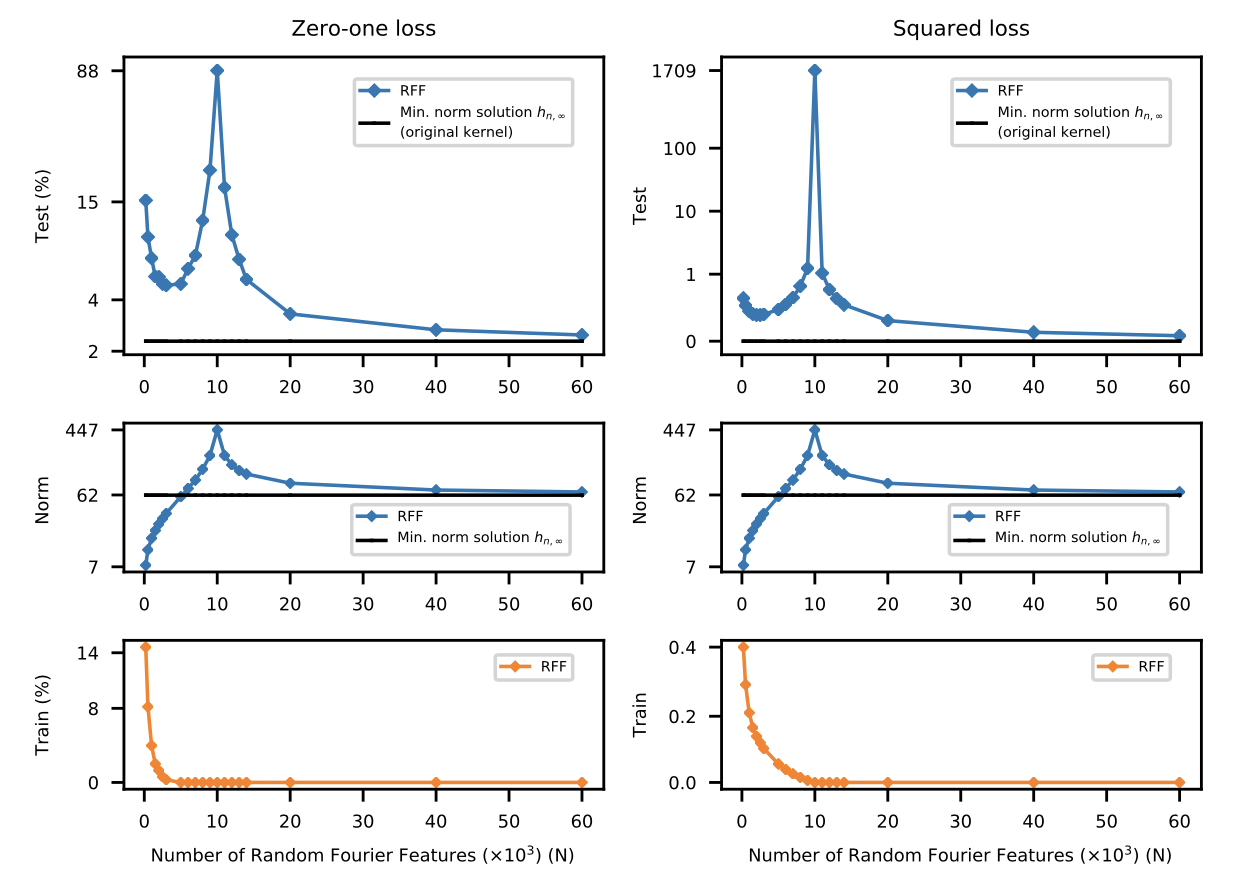
\includegraphics[height=0.39\textwidth]{belkin1.png}
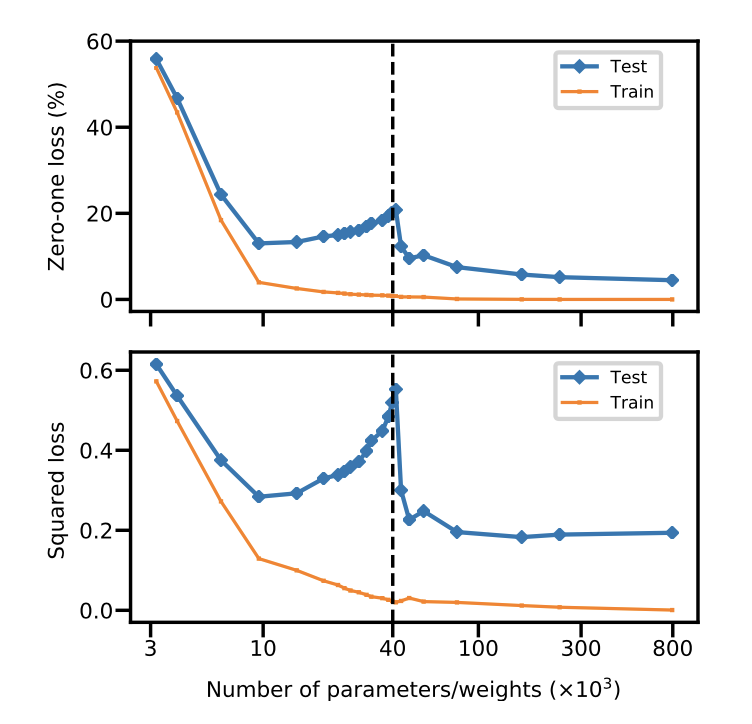
\includegraphics[height=0.39\textwidth]{belkin2.png} 
\bigskip\medskip \\
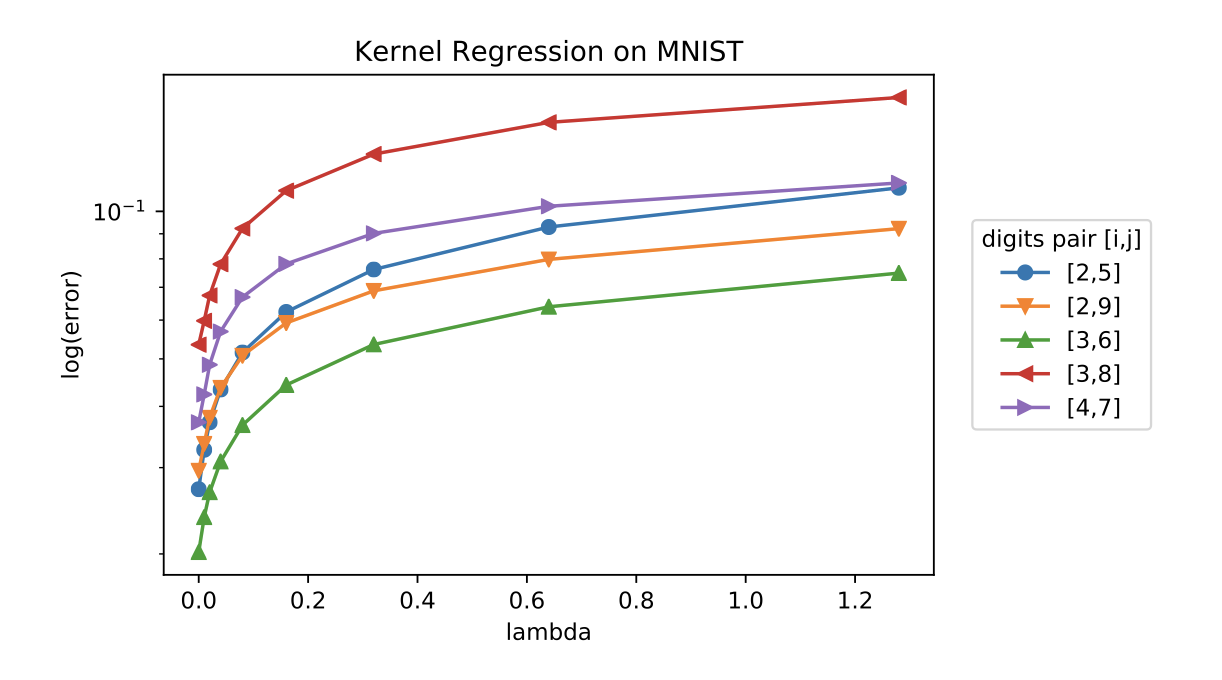
\includegraphics[width=0.69\textwidth]{liang.png} 
\bigskip \\
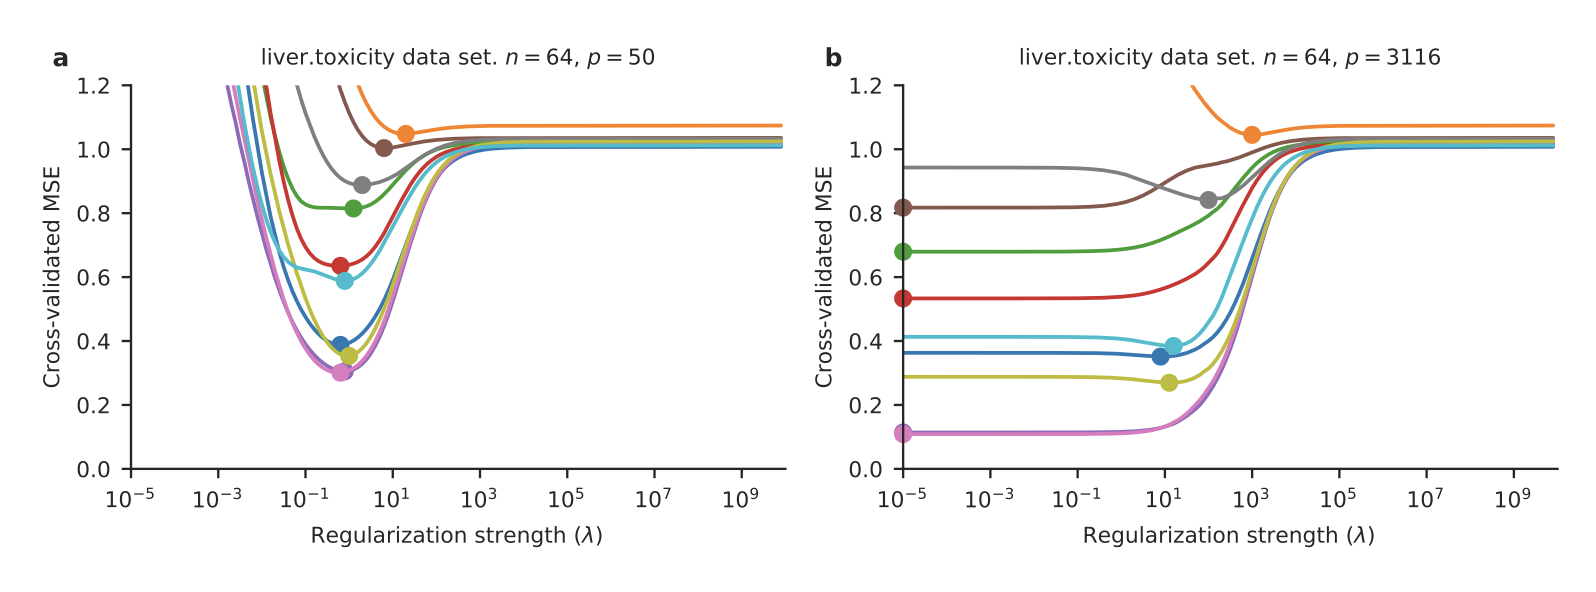
\includegraphics[width=0.98\textwidth]{kobak.png}
\caption{\it Experiments demonstrating the motivating points raised in the
  introduction. Interpolating estimators (with zero training error) can still   
  have good prediction error, as shown in the top row, credit:
  \citet{belkin2019reconciling}. Tuning over regularization levels can 
  suggest that vanishing regularization is optimal even in high 
  dimensions, as shown in the middle row, credit: \citet{liang2020just}, and
  bottom row, credit: \citet{kobak2020optimal}. The behavior of the prediction
  risk in the top row is dubbed ``double descent''.}   
\label{fig:experiments}
\end{figure}

\subsection{What's new here?}

Statisticians have been interested in high-dimensional models for a long
time. So what's new here? Don't the terms ``high-dimensional'' (in use for
several decades) and ``overparametrized'' (popularized recently) refer the same
thing?    

In a sense, the answer is both ``yes'' and ``no''. While traditional
high-dimensional analyses (like those we studied for the lasso) and newer
overparametrized analyses are clearly very related, they are also different in
some key ways. In the study of overparametrized models:
\begin{itemize}
\item we focus exclusively on out-of-sample prediction error---unlike many 
  traditional high-dimensional regression analyses which focus on in-sample
  prediction error (and treat out-of-sample prediction error as somewhat of an 
  afterthought);  
\item we care about how the risk landscape behaves as we vary the regularization  
  strength, and particularly what happens for vanishing explicit
  regularization---unlike many traditional analyses which study regimes where
  optimal performance is given by strong explicit regularization.   
\end{itemize}
There are arguably other differences, but those are two of the most salient ones 
for our discussion.

\subsection{Ridgeless least squares}

Given a response vector $Y \in \R^n$ and predictor matrix $X \in \R^{n \times
  d}$, as usual, we consider the \emph{minimum $\ell_2$ norm least squares} 
(or simply min-norm least squares) estimator,
\begin{equation}
\label{eq:ls_min}
\hbeta = (X^\T X)^+ X^\T Y,
\end{equation}
where $(X^\T X)^+$ denotes the Moore-Penrose pseudoinverse of $X^\T X$.
Equivalently, we can write this as
\[
\hbeta = \argmin \Big\{ \|\beta\|_2 : \beta \; \text{minimizes} \; \|Y - X
\beta\|_2^2 \Big\},   
\]
which explains its name.  

An alternative name for \eqref{eq:ls_min} is the ``ridgeless'' least squares
estimator. This is because it can be written as the limit of the ridge estimator
for vanishing regularization:  
\[
\hbeta = \lim_{\lambda \to 0} \, (X^\T X + \lambda I)^{-1} X^\T Y =   
\lim_{\lambda \to 0} \, \argmin_\beta \; \|Y - X\beta\|_2^2 + \lambda 
\|\beta\|_2^2.   
\]
When $X$ has rank $d$, the min-norm least squares estimator reduces to
\smash{$\hbeta = (X^\T X)^{-1} X^\T Y$}, the usual least squares estimator.
Importantly, when $X$ has rank $n$, this estimator interpolates the training 
data: \smash{$y_i = x_i^\T \hbeta$}, for $i=1,\dots,n$.   

\subsection{Connection to gradient descent}

There is an interesting connection between gradient descent and the min-norm
least squares estimator. Initialize $\beta^{(0)} = 0$, and consider running
gradient descent on the least squares loss, yielding iterates
\[
\beta^{(k)} = \beta^{(k-1)} + t X^\T (y-X\beta^{(k-1)}), 
\quad k=1,2,3,\dots,
\]
where we take the step size $t>0$ to be small enough. Then gradient descent
converges to the min-norm least squares solution in \eqref{eq:ls_min}:
\[
\lim_{k \to \infty} \, \beta^{(k)} = \hbeta.
\]
Why? It's quite simple: the updates \smash{$\beta^{(k)}$}, $k=1,2,3,\dots$
always lie in the row space of $X$; hence their limit (guaranteed to exist for
small enough $t>0$) must also lie in the row space of $X$; and the min-norm
least squares solution is the unique least squares solution with this property.    

The same result (and proof) carries over to stochastic gradient descent, and any 
other variants of gradient descent whose updates remain in the row space of $X$.  
Since these algorithms comprise the defacto standard for training neural
networks, one can argue that that minimum $\ell_2$ norm solutions arise
naturally as interesting objects of study based on practical conventions (and
successes) in machine learning.  

\section{Problem setup}

\def\asto{\overset{\mathrm{as}}{\to}}
\def\dto{\overset{d}{\to}}
\def\Risk{\mathrm{Risk}}
\def\Bias{\mathrm{Bias}}
\def\hSigma{\hat\Sigma}

We will assume the usual linear model 
\begin{equation}
\label{eq:model}
Y = X\beta_0 + \epsilon,
\end{equation}
where $\epsilon \in \R^n$ has i.i.d.\ entries with mean zero and variance
$\sigma^2$, and $\epsilon \indep X$. The conditions we will assume on the
features $X \in \R^{n \times d}$ are as follows:
\begin{itemize}
\item[(A1)] $X = Z \Sigma^{1/2}$, where the entries of $Z \in \R^{n \times d}$
  are i.i.d.\ with zero mean, unit variance, and finite $8+\eta$ moment, for
  some $\eta>0$; 
\item[(A2)] the covariance matrix $\Sigma \in \R^{d \times d}$ has eigenvalues
  bounded away from $0$ and $\infty$, and satisfies \smash{$F_\Sigma \dto H$},
  as $n,d \to \infty$; 
\item[(A3)] $d/n \to \gamma \in (1,\infty)$ as $n,d \to \infty$.
\end{itemize}
To emphasize, we are considering here $\gamma > 1$, called the
\emph{overparametrized} regime. As in the ridge lecture, we will be interested
in the out-of-sample prediction risk, conditional on $X$, 
\begin{equation}
\label{eq:risk}
\Risk_X(\hbeta; \beta_0) = \E \big[ ( x_0^\T \hbeta - x_0^\T \beta_0 )^2
\,\big|\, X \big],
\end{equation}
where $x_0 = \Sigma^{1/2} z_0$ is i.i.d.\ to the rows of $X$. We will study the
risk of min-norm least squares in \eqref{eq:ls_min}. 

\subsection{Summary}

Here is a summary of what will happen in linear models, based roughly on the
development of results  in \citet{hastie2022surprises}. At the outset, we should
note that there are a lot of other interesting results from other recent papers
that we will not be covering. This includes some work that goes beyond linear
feature models and budges closer what actually happens in neural networks. For
nice surveys on the recent explosion of work on overparametrization theory, see 
\citet{bartlett2021deep, belkin2021fit, dar2021farewell}.      

\begin{enumerate}
\item[0.]
In the underparametrized regime ($\gamma < 1$), the risk is purely variance
(there is no bias), and does not depend on $\beta_0$ or $\Sigma$. Indeed, recall
that we already showed in the last lecture that
\begin{equation}
\label{eq:ls_risk_limit}
\Risk_X(\hbeta; \beta_0) \asto \sigma^2 \frac{\gamma}{1-\gamma}.
\end{equation}
This blows up as $\gamma \to 1$ from below. 

\item
In the overparametrized regime ($\gamma > 1$), the risk is composed of both
bias and variance, and generally depends on $\Sigma$ or $\beta_0$. The
asymptotic risk descends from its asymptote at $\gamma = 1$, but there is no
longer a simple explicit formula that describes its behavior with $\gamma$ in
full generality.

\item
In the isotropic case $\Sigma = I$, we can derive a simple formula for the
limiting risk for fixed $\beta_0$. This case already exhibits some interesting
and informative properties. For example, in a misspecified model (where the mean
$\E[y_i|x_i]$ is no longer linear in $x_i$ in \eqref{eq:model}), the risk can
attain its global minimum at $\gamma \in (1,\infty)$. 

However, this case fails to shed light on other important aspects that we seek
to understand; in particular, optimal regularization strength in ridge
regression in this isotropic case is always be positive.

\item
In the case of general $\Sigma$, we can derive an explicit formula for the
asymptotic variance. As in the ridge analysis, this is no longer closed-form,
but still we can learn various things. For example, in specific covariance
structures, we can study the variance term as a function of correlation
strength.    

The behavior of the bias is much more complex. With a prior on $\beta_0$, we can 
get back an explicit asymptotic formula (as in the ridge lecture), but this
again fails to shed light on important aspects we would like to study, as
optimal regularization strength in ridge regression is again always positive.     

\item
Thus to expose when and how ridgeless regularization ($\lambda \to 0$) can be
optimal, we must study the bias for general $\Sigma$, and fixed $\beta_0$. This
is a lot more challenging, but it can be done. The optimality of ridgeless 
regularization can rigorously confirmed in a latent space model (which is a kind
of misspecified model). 

\item
Finally, though still much more challenging, concrete progress can be made
outside of the linear feature model. In certain nonlinear settings, some aspects
of the lessons from linear feature models are preserved. You'll explore this 
(numerically) on the homework.  
\end{enumerate}

\subsection{Plan-of-attack?}

In general, there are two ways to proceed to derive the risk of the ridgeless
regression estimator \eqref{eq:ls_min}. The first is to take asymptotic results
for ridge regression (such as those we derived in the previous lecture) and then
let $\lambda \to 0$, which typically requires us to be careful about how to
resolve indeterminate limits. 

The second is to start with the bias and variance expressions for min-norm 
least squares, and then carry out asymptotic calculations directly. Often, these
calculations require us to ``ridge-ify'' some of the matrix functionals
that involve pseudoinverses, and then let the auxiliary ridge parameter tend to
zero. Curiously, the ``ridge-ified'' functionals in the second approach are not
always exactly the same as those that appear in the asymptotic calculations for
ridge regression, and the former can sometimes be easier to analyze in the
ridgeless limit (of course we must end up with the same answers at the end with
either approach).   

We will generally follow the second plan-of-attack, if only to give you more
exposure to the elegant and powerful nature of random matrix theory. (Though to
be frank in what follows we will only really cover the proof details for the 
isotropic case.) In preparation for this, it is helpful to rewrite the ridgeless
estimator  \eqref{eq:ls_min} as \smash{$\hbeta = (X^\T X/n)^+ X^\T Y/n$}, and
helpful to record the bias and variance components of its risk:  
\begin{align}
\label{eq:ls_min_bias}
\Bias_X(\hbeta; \beta_0) &= \beta_0^\T (I - \hSigma^+ \hSigma) \Sigma 
  (I - \hSigma^+ \hSigma) \beta_0 \\  
\label{eq:ls_min_var}
\Var_X(\hbeta) &= \frac{\sigma^2}{n} \tr (\hSigma^+ \Sigma),
\end{align}
where \smash{$\hSigma = X^\T X/n$}, which follows from calculations similar to
those in the underparametrized case.      

\section{Isotropic $\Sigma$, fixed $\beta_0$}

We consider the isotropic case, $\Sigma = I$.  We will assume that $\|\beta_0\|_2
= r$ (which is a constant that does not vary with $n,d$), for the true signal
vector in \eqref{eq:model}. Below we analyze the bias and variance separately.

\paragraph{Bias analysis.}

When $\Sigma = I$, the bias \eqref{eq:ls_min_bias} becomes 
\begin{align}
\nonumber
\Bias_X(\hbeta; \beta_0) 
&= \beta_0^\T (I - \hSigma^+ \hSigma) \beta_0 \\ 
\nonumber
&= \lim_{\rho \to 0} \, \beta_0^\T \big[ I - (\hSigma + \rho I)^{-1} \hSigma  
  \big] \beta_0 \\   
\label{eq:ls_min_bias_iso}
&= \lim_{\rho \to 0} \, \rho \beta_0^\T (\hSigma + \rho I)^{-1} \beta_0,  
\end{align}
where in the second line we used the general fact \smash{$(A^\T A)^+ A^\T =
  \lim_{\rho \to 0} \, (A^\T A + \rho I)^{-1} A^\T$}, to \smash{$A =
  X/\sqrt{n}$}, and in the third line we added and subtracted $\rho I$ to
trailing \smash{$\hSigma$} in the matrix product. (All limits $\rho \to 0$ here  
and henceforth are to be interpreted as from above.) 

By the generalized MP theorem from \citet{rubio2011spectral} (transcribed in
Theorem 2 in the ridge lecture notes using the language of deterministic
equivalents), we know that  
\[
\beta_0^\T (\hSigma + \rho I)^{-1} \beta_0 \quad \text{and} \quad 
\beta_0^\T (a_n I + \rho I)^{-1} \beta_0 = \frac{r^2}{a_n + \rho} \quad
\text{have the same asymptotic limit},
\]
where $a_n$ satisfies a certain fixed-point equation. To compute the limit of
$a_n$, we note that also
\[
\frac{1}{d} \tr \big[ (\hSigma + \rho I)^{-1} \big] \quad \text{and} \quad  
\frac{1}{d} \tr \big[ (a_n I + \rho I)^{-1} \big] = \frac{1}{a_n + \rho}
\quad \text{have the same asymptotic limit},  
\]
and by the standard MP asymptotics, the left-hand side converges almost surely
to $m_F(-\rho)$, the Stieltjes transform of the MP law, evaluated at
$-\rho$. Thus we have $1/(a_n + \rho) \to m_F(-\rho)$, and    
\[
\beta_0^\T (\hSigma + \rho I)^{-1} \beta_0 \asto r^2 m_F(-\rho). 
\]
Returning to \eqref{eq:ls_min_bias_iso}, some calculations involving the
Moore-Osgood theorem (whose details we omit) allow us to switch the order of the
limits as $n,d \to \infty$ and $\rho \to 0$, yielding
\begin{align}
\nonumber
\Bias_X(\hbeta; \beta_0) &\asto r^2 \lim_{\rho \to 0} \, \rho \, m_F(-\rho) \\
\nonumber
&= r^2 \lim_{\rho \to 0} \, \frac{-(1 - \gamma + \rho) + \sqrt{(1 - \gamma +
  \rho)^2 + 4 \gamma \rho}}{2 \gamma} \\
\nonumber
&= r^2 \frac{-(1-\gamma) + (\gamma-1)}{2 \gamma} \\
\label{eq:ls_min_bias_iso_limit}
&= r^2 \Big( 1- \frac{1}{\gamma} \Big),
\end{align}
where to compute the limit we have used the explicit form of the Stieltjes
transform of the MP law (as covered in the ridge lecture notes).

\paragraph{Variance analysis.}

When $\Sigma = I$, the variance analysis is actually quite easy (relatively
speaking). From \eqref{eq:ls_min_var}, we have
\[
V_X(\hbeta; \beta_0) = \sigma^2 \sum_{i=1}^n \frac{1}{s_i(X^\T X)},
\]
where $s_i(X^\T X/n)$, $i=1,\dots,n$ denote the nonzero eigenvalues of $X^\T  
X/n$. Then because $X^\T X$ and $XX^\T$ always have the same nonzero
eigenvalues, we may write this as
\[
V_X(\hbeta; \beta_0) = \sigma^2 \sum_{i=1}^n \frac{1}{s_i(X^\T X)} = 
\frac{\sigma^2 n}{d} \frac{1}{n} \tr\big[ (XX^\T /d)^{-1} \big].
\]
The rightmost term above is precisely the form of the variance in the
underparametrized case, but with $X^\T$ in place of $X$. Thus, denoting $\tau =
n/d < 1$, we conclude from our previous analysis that  
\begin{equation}
\label{eq:ls_min_var_iso_limit}
V_X(\hbeta; \beta) \asto \sigma^2 \frac{\tau}{1-\tau} = \sigma^2 
\frac{1}{\gamma-1},  
\end{equation}

\paragraph{Putting it together.}

Adding the bias \eqref{eq:ls_min_bias_iso_limit} and variance results
\eqref{eq:ls_min_var_iso_limit} together, we get
\begin{equation}
\label{eq:ls_min_risk_iso_limit}
\Risk_X(\hbeta; \beta_0) \asto r^2 \Big( 1- \frac{1}{\gamma} \Big) + \sigma^2 
\frac{1}{\gamma-1}. 
\end{equation}
This has quite a striking profile:
\begin{quote}
\centering\it
The out-of-sample risk of least squares descends from its asymptote at the
interpolation threshold $\gamma = 1$. The bias grows with $\gamma$, but 
the variance decreases with $\gamma$.      
\end{quote}
The calculation above explains why the variance decreases with $\gamma$: we
found that the variance of min-norm least squares on $n$ samples and $d$
features is precisely the variance of \emph{ordinary} least squares on $d$
samples and $n$ features. See Figure \ref{fig:risk_iso} for visualization of the
risk profile over $\gamma$.

\begin{figure}[htb]
\centering
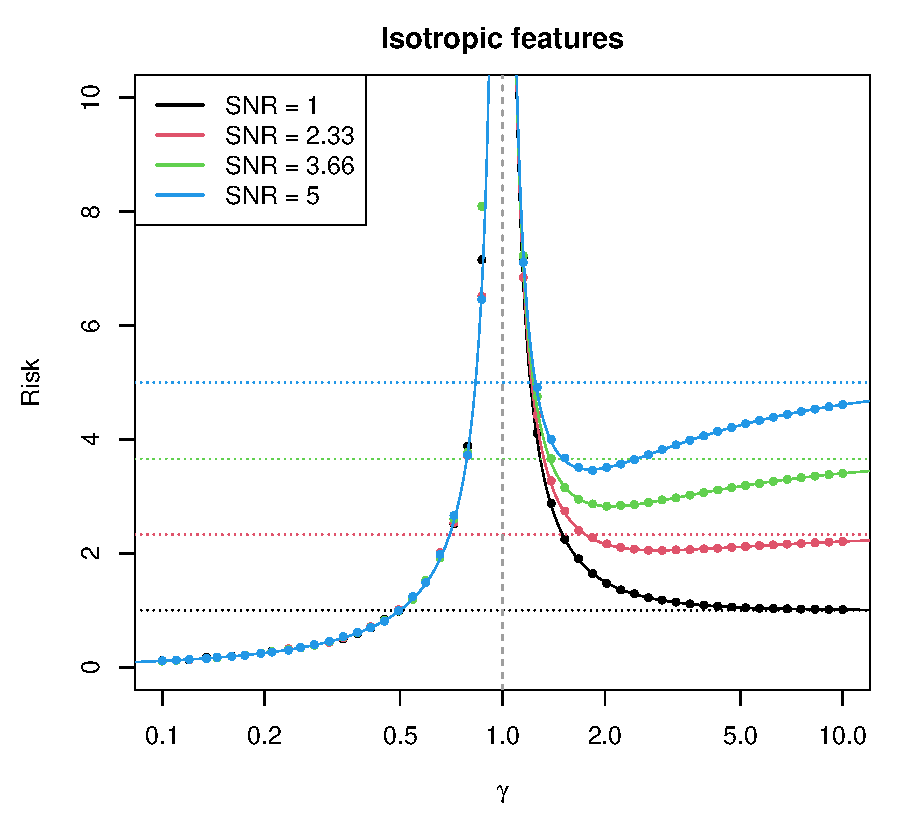
\includegraphics[width=0.6\textwidth]{risk_iso.pdf}
\caption{\it The asymptotic risk of least squares \eqref{eq:ls_risk_limit} for
  $\gamma<1$ and min-norm least squares \eqref{eq:ls_min_risk_iso_limit} for
  $\gamma>1$, where the latter assumes $\Sigma = I$, the isotropic
  case. Different colors represent different values of $\mathrm{SNR} = r^2 /
  \sigma^2$. The points denote finite-sample risks, computed from i.i.d.\
  standard Gaussian features with $n=200$ and $d=[\gamma n]$ for varying
  $\gamma$. Credit: \citet{hastie2022surprises}.}  
\label{fig:risk_iso}
\end{figure}

\section{Misspecified setting}

The latter analysis portrays an interesting feature of ridgeless regression in  
the overparametrized regime: its variance is well-controlled past the
interpolation threshold $\gamma = 1$. However, it fails to exhibit any real
benefit to doing ridgeless regression in the overparametrized regime, because
the global minimum of the risk is always at $\gamma = 0$. We also do not see
double descent in Figure \ref{fig:risk_iso}, as the first descent over $\gamma
\in (0,1)$ never happens. This is due to the fact that we are assuming, for any 
$n,d$, a true linear model in $d$ features, which makes it hard to reason about
what happens across different dimensions $d$.    

We therefore pursue a small but important change to the model in
\eqref{eq:model}: we instead assume that    
\begin{equation}
\label{eq:model_mis}
Y = X\beta_0 + W\theta_0 + \epsilon,
\end{equation}
Everything is the same as before, with respect to the distributions of $X$ and
$\epsilon$. But now we have an additional part of the mean function that is
driven by $W$, which we treat as a matrix of \emph{unobserved} features (that we 
do not have in hand). Thus we still just carry out regression of $Y$ on $X$, as
in \eqref{eq:ls_min}. In this context, we call \eqref{eq:model_mis} a
\emph{misspecified} model, and analogous to \eqref{eq:risk}, we are now
interested in risk defined as:
\begin{equation}
\label{eq:risk_mis}
\Risk_X(\hbeta; \beta_0, \theta_0) = \E \big[ \big( x_0^\T \hbeta -
\E[y_0|x_0,w_0] \big)^2 \,\big|\, X \big],
\end{equation}
where $(x_0,w_0,y_0)$ is an i.i.d.\ draw from the same joint distribution as in 
\eqref{eq:model_mis}. 

\subsection{Risk decomposition} 

We can always write 
\begin{equation}
\label{eq:risk_mis_decomp}
\Risk_X(\hbeta; \beta_0, \theta_0) = 
\underbrace{\E \big[ \big( x_0^\T \hbeta - \E[y_0|x_0] \big)^2 \,|\, X 
  \big]}_{L_X(\hbeta; \beta_0, \theta_0)} +
\underbrace{\E \big[ \big( \E[y_0|x_0] - \E[y_0|x_0,w_0] \big)^2
  \big]}_{M(\beta_0, \theta_0)}, 
\end{equation}
which is verified by simply verified by first conditioning on $x_0$, then adding
an subtracting $\E[y_0|x_0]$ inside the square in the definition of
\smash{$R_X(\hbeta; \beta_0, \theta_0)$} in \eqref{eq:risk_mis}, and expanding, 
and noting that the cross term is zero:   
\[
\E \big[ \big( x_0^\T \hbeta - \E[y_0|x_0] \big) \,|\, X,x_0 \big]
\E \big[\big( \E[y_0|x_0] - \E[y_0|x_0,w_0] \big) \,|\, x_0 \big] = 0.
\]

In other words, from \eqref{eq:risk_mis_decomp}, we learn that the risk in the
misspecified setting decomposes into two terms: \smash{$L_X(\hbeta; \beta_0,
  \theta_0)$}, measuring how well we can predict the conditional mean of
$\E[y_0|x_0]$, and \smash{$M_X(\hbeta; \beta_0, \theta_0)$}, measuring how far
apart $\E[y_0|x_0]$ and $\E[y_0|x_0,w_0]$ are. We call the latter term the
\emph{misspecification bias} (note that it does not depend at all on $X$ or
\smash{$\hbeta$}).   

\subsection{Simplest analysis}

In the simplest case, we can take the distribution of the unobserved features
$W$ to be independent of $X$ (and $\epsilon$), with the covariances of $X,W$
each being the identity---in keeping with the isotropic setting just
studied. This allows to rewrite \eqref{eq:risk_mis} as 
\[
Y = X\beta_0 + \delta,
\]
where the entries of $\delta = W\theta_0 + \epsilon$ are still i.i.d.\ with mean
zero, and their variance is $\|\theta_0\|_2^2 + \sigma^2$. Denote 
\[
r^2=\|\beta_0\|_2^2+\|\theta_0\|_2^2 \quad \text{and} \quad 
\kappa=\|\beta_0\|_2^2 / r^2,
\]
which represents the total signal energy and the the fraction of the signal
energy captured by the observed features, respectively. Then \smash{$L_X(\hbeta;
  \beta_0, \theta_0)$} behaves exactly as we computed previously, in
\eqref{eq:ls_risk_limit} for $\gamma<1$ and \eqref{eq:ls_min_risk_iso_limit} for
$\gamma>1$, after we make the substitutions:     
\[
r^2 \mapsto r^2 \kappa \quad \text{and} \quad
\sigma^2 \mapsto \sigma^2 + r^2 (1-\kappa).
\]
Furthermore, we can easily calculate the misspecification bias as: 
\[
M(\beta_0, \theta_0) = \E[(w_0^\T \theta_0)^2] = r^2 (1-\kappa). 
\]
Putting these results together leads to the following conclusion:
\begin{equation}
\label{eq:ls_min_risk_iso_mis_limit}
\Risk_X(\hbeta; \beta_0; \theta_0) \asto 
\begin{cases}
r^2(1-\kappa) + \big(r^2(1-\kappa) + \sigma^2\big) 
\frac{\gamma}{1-\gamma} & \text{for $\gamma < 1$}, \\
r^2(1-\kappa) + r^2 \kappa \big(1-\frac{1}{\gamma}\big) 
+ \big(r^2(1-\kappa) + \sigma^2\big) \frac{1}{\gamma-1} &  
\text{for $\gamma > 1$}.
\end{cases}
\end{equation}

\subsection{Interpretation}

To interpret the risk profiles \eqref{eq:ls_min_risk_iso_mis_limit} in the
misspecified setting, we will need to specify a relationship between $\kappa$
and $\gamma$. Since adding features should generally improve our approximation
capacity, it is reasonable to model $\kappa=\kappa(\gamma)$ as an increasing 
function of $\gamma$. Figure \ref{fig:risk_iso_mis} gives an example with a
polynomial decay, $1-\kappa(\gamma) = (1+\gamma)^{-a}$. Notably, we can see a
clear double descent in the risk curve, and for certain values of $a$ (such as
that plotted in green), we find that the global min of the risk occurs at
$\gamma > 1$.  

\begin{figure}[htb]
\centering
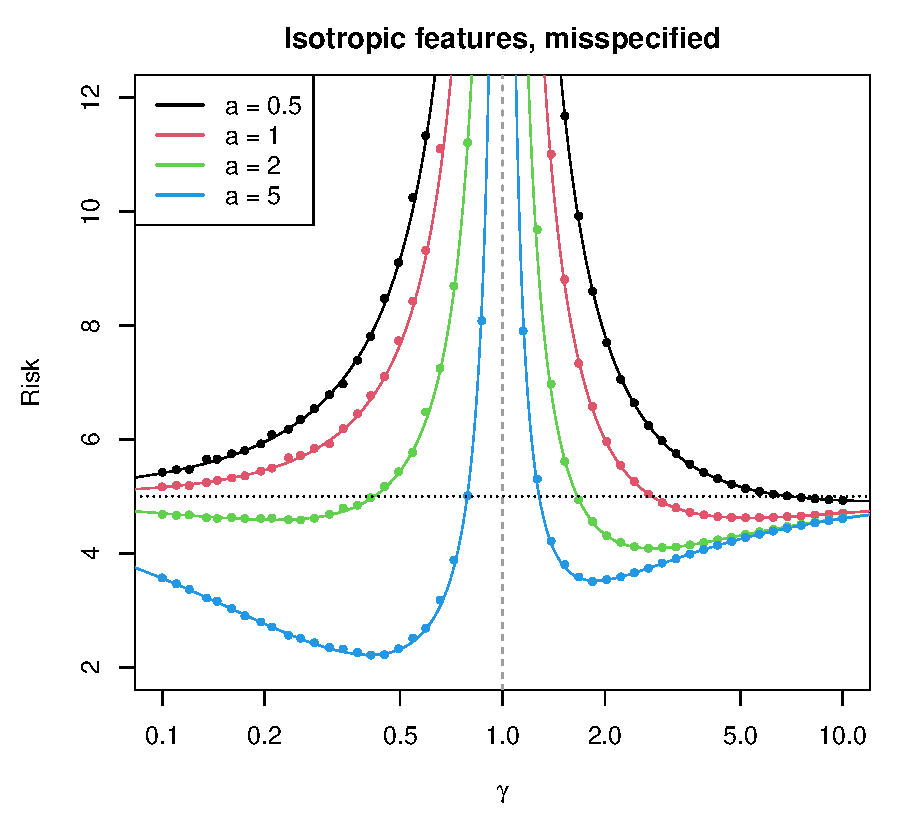
\includegraphics[width=0.6\textwidth]{risk_iso_mis.pdf}
\caption{\it The asymptotic risk of min-norm least squares in the misspecified
  setting \eqref{eq:ls_min_risk_iso_mis_limit}, with isotropic observed and
  unobserved feature covariances, and $1-\kappa(\gamma) = (1+\gamma)^{-a}$. We
  set $\mathrm{SNR} = r^2 / \sigma^2 = 5$. Different colors represent different
  values of $a$. As in Figure \ref{fig:risk_iso}, the points denote
  finite-sample risks, computed from $n=200$ and $d=[\gamma n]$ for varying 
  $\gamma$. Credit: \citet{hastie2022surprises}.}   
\label{fig:risk_iso_mis}
\end{figure}

As a concluding remark in this misspecified setting, we note that the dimension
of the unobserved features (the number of columns of $W$) enters nowhere in
these calculations, so we can effectively think of it as infinite. This provides
us with a nice interpretation: we have an infinitely wide matrix $[X; W]$ that 
governs the behavior of $Y$ in the model \eqref{eq:model}. As $d$ grows, we
observe more and more columns of this matrix, which improves our approximation
capacity. This is an analogy to what a feature generator can do for us.       

\section{General $\Sigma$, random $\beta_0$}

In the general $\Sigma$ case, just as in the ridge analysis, the bias in 
\eqref{eq:ls_min_bias} is especially difficult to calculate. We can make
progress by placing a spherical prior on $\beta_0$, such that        
\begin{equation}
\label{eq:prior}
\E[\beta_0 \beta_0^\T] = \frac{r^2}{d} I.
\end{equation}

\paragraph{Bias analysis.}

By similar arguments to those in the isotropic case above and the ridge lecture,
whose details we omit, one can show that for the Bayes bias, given by
integrating \eqref{eq:ls_min_bias} over $\beta_0$,
\begin{equation}
\label{eq:ls_min_bias_bayes_limit}
\Bias_X(\hbeta) \asto \frac{r^2}{\gamma} \frac{1}{v_F(0)},  
\end{equation}
where $v_F$ is the companion Stieltjes transform of the limiting spectral
distribution $F = F(H, \gamma)$ from the Marchenko-Pastur theorem (and
\smash{$v_F(0) = \lim_{\rho \to 0} \, v_F(-\rho)$} exists under our
assumptions).   

\paragraph{Variance analysis.}

Again by similar arguments to those in the isotropic case and the ridge lecture,
whose details we also omit, one can show that for the variance in
\eqref{eq:ls_min_var},  
\begin{equation}
\label{eq:ls_min_var_limit}
\Var_X(\hbeta) \asto \sigma^2 \bigg(\frac{v'_F(0)}{v_F(0)^2} - 1 \bigg),
\end{equation}
where again $v_F$ is the companion Stieltjes transform of the limiting spectral 
distribution $F = F(H, \gamma)$ from the MP theorem (and
\smash{$v'_F(0)/v_F(0)^2 = \lim_{\rho \to 0} \, v'_F(-\rho)/v_F(-\rho)^2$}
exists under our assumptions). We emphasize that the variance calculation in 
\eqref{eq:ls_min_var_limit} does not depend on the prior \eqref{eq:prior} and is
fully general.    

\paragraph{Inspecting the asymptotics.}

We note that the some of the key dependence of
\eqref{eq:ls_min_bias_bayes_limit}, \eqref{eq:ls_min_var_limit} on $\gamma$ is
hidden in the Stieltjes transform terms $v_F(0)$, $v'_F(0)$, which themselves
depends on $\gamma$ (since $F$ does). While these asymptotic limit cannot be
computed in closed-form for general covariance models (general $H$), they can be
computed numerically by solving the Silverstein equation. This is done in
\citet{hastie2022surprises}, in order to probe the asymptotic limits, and better
understand how they behave. This reveals some interesting phenomena, such as 
the fact that stronger correlations can increase the variance, but decrease the
Bayes bias. See Figure \ref{fig:risk_ec_ar}. 

\begin{figure}[p]
\centering
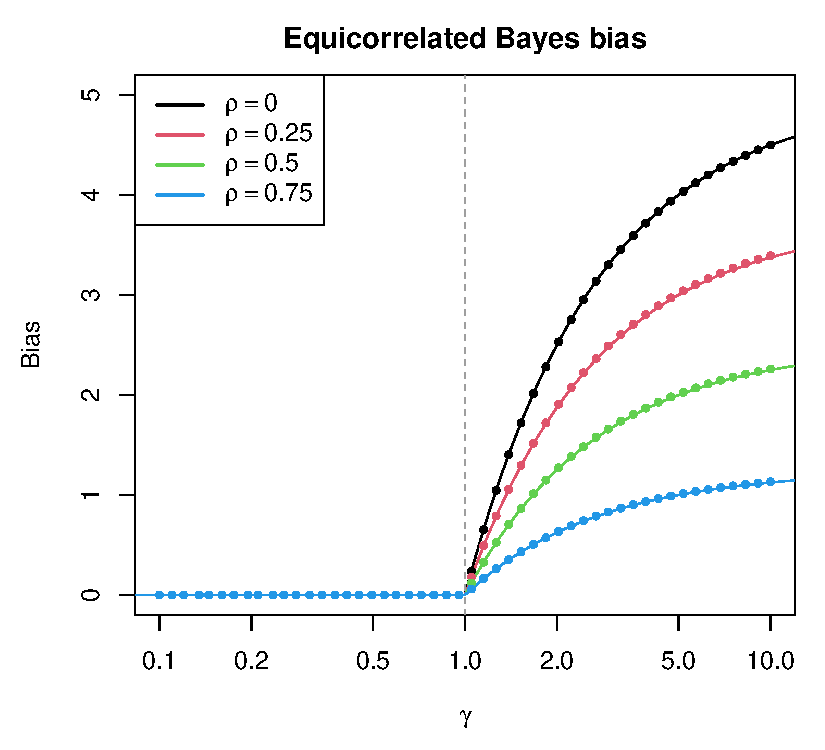
\includegraphics[width=0.49\textwidth]{bias_ec.pdf}
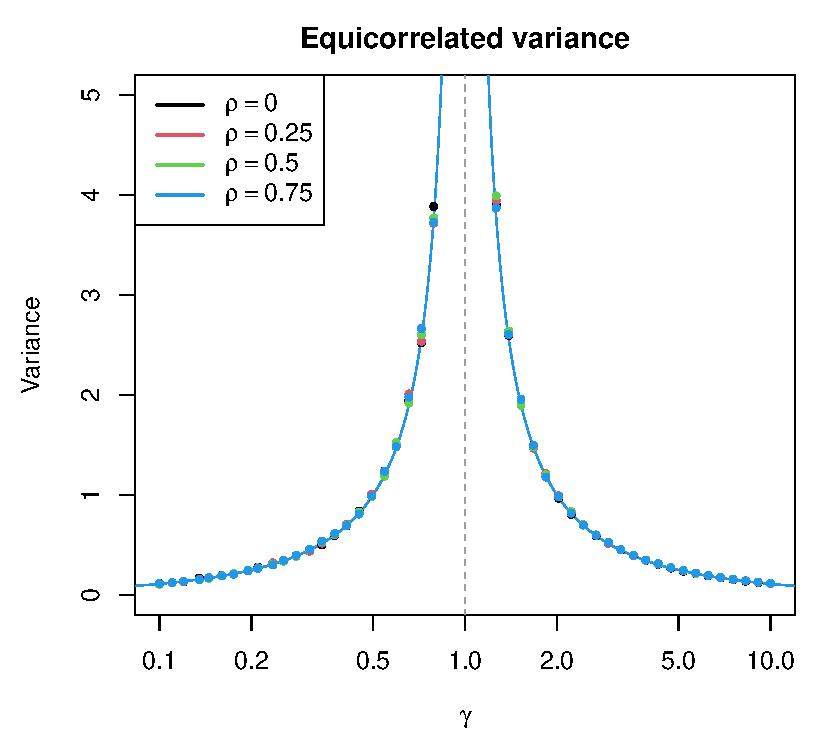
\includegraphics[width=0.49\textwidth]{var_ec.pdf}
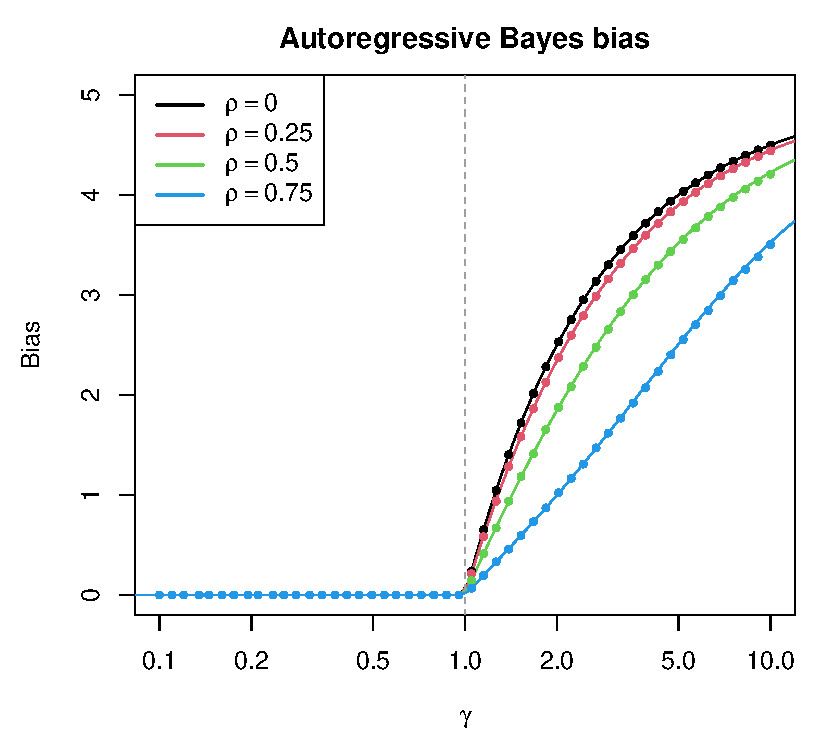
\includegraphics[width=0.49\textwidth]{bias_ar.pdf}
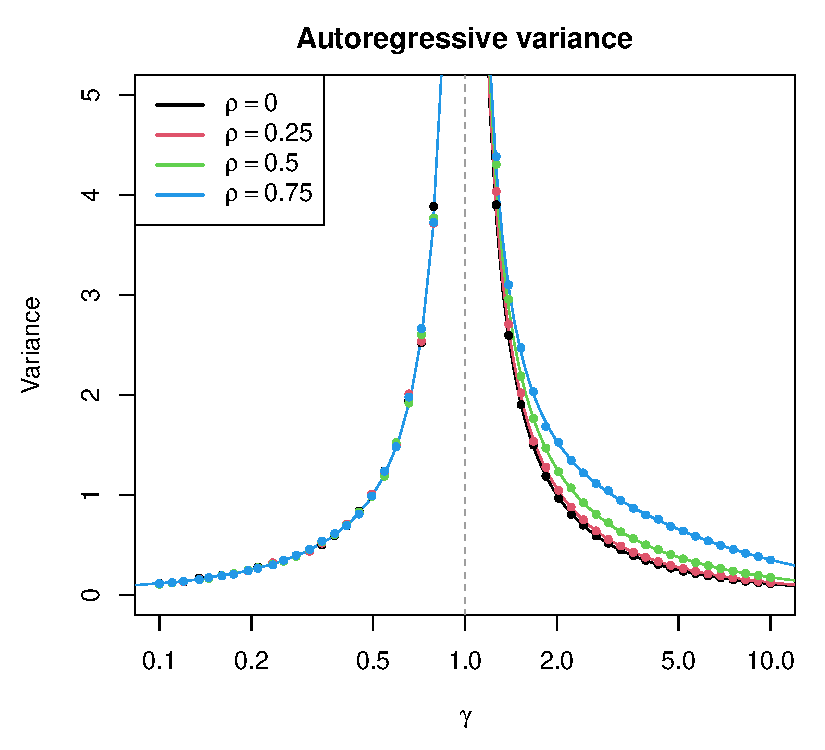
\includegraphics[width=0.49\textwidth]{var_ar.pdf}
\caption{\it Asymptotic Bayes bias and variance of min-norm least squares for
  different feature covariance models. The top row shows an equicorrelated
  feature model, where $\Sigma_{ij} = 1$ if $i=j$ and $\rho$ otherwise. In this 
  model the asymptotics can be done in closed-form: we find the bias decreases
  with $\rho$, whereas the variance does not actually depend on $\rho$. The
  bottom row shows an autocorrelated feature model, where $\Sigma_{ij} = 
  \rho^{|i-j|}$. Here the asymptotics cannot be done in closed-form but they can  
  be efficiently computed numerically: we find that the bias decreases with
  $\rho$, and the variance increases with $\rho$. Credit:
  \citet{hastie2022surprises}.}      
\label{fig:risk_ec_ar}
\end{figure}

\paragraph{Where this fall short.}

The Bayes model studied here falls short in one key way. It does not explain why
ridgeless regression is statistically interesting above and beyond ridge
regression. In the Bayes model studied here, recall (from the last lecture), we
know that the asymptotically optimal ridge tuning parameter is $\lambda^* =
\sigma^2 \gamma / r^2$, regardless of the feature covariance model. This is
always positive, and depends only on the SNR. Thus in order to really understand
the phenomena in Figure \ref{fig:experiments}, i.e., to understand when and how
the ridge risk landscape can be minimized at $\lambda = 0$, we must tackle the
beast: calculate the ridge bias for general $\Sigma$ and fixed $\beta_0$.     

\section{General $\Sigma$, fixed $\beta_0$}

For general $\Sigma$, and a fixed $\beta_0$, the ridge bias where (recall)
\smash{$\hbeta_\lambda = (X^\T X + n \lambda I)^{-1} X^\T Y$} for $\lambda>0$,
and  
\begin{equation}
\label{eq:ridge_bias}
\Bias_X(\hbeta_\lambda; \beta_0) = \lambda^2 \beta_0^\T (\hSigma + \lambda
I)^{-1} \Sigma (\hSigma + \lambda I)^{-1} \beta_0,
\end{equation}
and especially the ridgeless bias \eqref{eq:ls_min_bias}, are formidable
calculations.   

The variance calculations in the ridge or ridgeless risk expansions that we
computed in the previous general $\Sigma$ analyses (in the ridge lecture, and in
the last section) were done under the guise of a prior assumption on $\beta_0$,
but this assumption did not actually matter for the variance terms, so they were
already carried out in full generality anyway.     

For the ridge bias, the main challenge is that the functional \smash{$(\hSigma + 
  \lambda I)^{-1} \Sigma (\hSigma + \lambda I)^{-1}$} does not has a transparent
deterministic equivalent; and similarly for the ridgeless bias. Only recently
have results started to appear on the asymptotics of the ridge and ridgeless
bias terms for general $\Sigma$ and $\beta_0$, see, e.g., \citet{wu2020optimal, 
  richards2021asymptotics, hastie2022surprises}. We mainly follow the
calculations in the latter paper (as they are, in a sense, the most general
anyway), but in keeping with our style in these lectures thus far, we translate
them to the language of deterministic equivalents. We only give some part of the
details; for the remainder, see the supplementary notes posted on the course
website.   

\paragraph{Ridge bias analysis.}

We start with the ridge bias calculation. We seek to use the generalized
Marchenko-Pastur theorem from \citet{rubio2011spectral} (Theorem 2 in the ridge
lecture notes), but it is not as of yet clearly applicable. There is one key
trick: we rewrite \eqref{eq:ridge_bias} as
\begin{equation}
\label{eq:deriv_trick}
\lambda^2 (\hSigma + \lambda I)^{-1} \Sigma (\hSigma + \lambda I)^{-1} = 
-\frac{d}{d\rho} \bigg\{ \lambda (\hSigma + \lambda I + \rho \lambda 
\Sigma)^{-1} \bigg\} \bigg|_{\rho=0}.  
\end{equation}
Note that this is similar in spirit to the way we have ``ridge-ified'' various
functionals above that involve pseudoinverses, but it is technically different:
the auxiliary parameter $\rho$ now multiplies $\lambda \Sigma$ (instead of simply
multiplying the identity matrix, as above). Checking \eqref{eq:deriv_trick} can
be done using the following general fact from matrix calculus: 
\begin{equation}
\label{eq:matrix_inv_deriv}
\frac{dA^{-1}}{d\rho} = - A^{-1} \frac{dA}{d\rho} A^{-1},
\end{equation}
for an invertible matrix $A$ (where $dA/d\rho$ is to be understood
elementwise). We can thus seek to compute a deterministic equivalent for the
functional inside the derivative on the right-hand side in
\eqref{eq:deriv_trick}, then differentiate with respect to $\rho$ and setting 
$\rho=0$. 

Towards this end, we rewrite it once more
\begin{align}
\nonumber
\lambda (\hSigma + \lambda I + \rho \lambda \Sigma)^{-1} 
&= \lambda \bigg( \Sigma^{1/2} \frac{Z^\T Z}{n} \Sigma^{1/2} + 
  \lambda (I + \rho \Sigma) \bigg)^{-1} \\
\label{eq:ridge_bias_wip1} 
&= (I + \rho \Sigma)^{-1/2} \lambda (\hSigma_\rho + \lambda I)^{-1} 
  (I + \rho \Sigma)^{-1/2},
\end{align}
where we define
\[
\hSigma_\rho = \Sigma_\rho^{1/2} \frac{Z^\T Z}{n} \Sigma_\rho^{1/2} 
\quad \text{and} \quad 
\Sigma_\rho = (I + \rho \Sigma)^{-1/2} \Sigma (I + \rho \Sigma)^{-1/2}. 
\]
Now the middle term in \eqref{eq:ridge_bias_wip1} has a deterministic equivalent 
by the generalized MP theorem,  
\begin{equation}
\label{eq:ridge_bias_wip2}
\lambda (\hSigma_\rho + \lambda I)^{-1} \asymp (c_n\Sigma_\rho + I)^{-1},
\end{equation}
where $c_n$ solves a particular fixed-point equation. Some calculations
(detailed in the supplementary notes) show that, after differentiating
\eqref{eq:ridge_bias_wip2} with respect to $\rho$ and taking $\rho=0$, we get 
the following conclusion: assuming $\|\beta_0\|_2$ remains bounded, the ridge
bias in \eqref{eq:ridge_bias} satisfies
\begin{equation}
\label{eq:ridge_bias_limit}
\big| \Bias_X(\hbeta_\lambda; \beta_0) - (1+c_n) \beta_0^\T \Sigma (b_n \Sigma + 
I)^{-2} \beta_0 \big| \asto 0, 
\end{equation}
where $b_n,c_n$ solve (recalling $\gamma_n = d/n$): 
\begin{align}
\label{eq:ridge_bn}
\frac{1}{b_n} &= \lambda + \frac{\gamma_n}{d} \tr \big[ \Sigma (b_n \Sigma +
  I)^{-1} \big]\\  
\label{eq:ridge_cn}
c_n &= \frac{\gamma_n \tr [ \Sigma^2 (b_n \Sigma + I)^{-2} ] / d}
{b_n^{-2} - \gamma_n \tr [ \Sigma^2 (b_n \Sigma + I)^{-2} ] / d}.
\end{align}
There are different parametrizations available for these fixed-point equations
(more later) but we choose to use the one above because it allows to send
$\lambda \to 0$ in a graceful way, which we do next.

\paragraph{Ridgeless bias analysis.}

To derive ridgeless asymptotics, we let $\lambda \to 0$ in
\eqref{eq:ridge_bias_limit}, \eqref{eq:ridge_bn}, \eqref{eq:ridge_cn} and defer
the details (on why this is valid) to the supplement. This yields for the
ridgeless estimator \smash{$\hbeta = (X^\T X)^+ X^\T Y$},
\begin{equation}
\label{eq:ridgeless_bias_limit}
\big| \Bias_X(\hbeta; \beta_0) - (1+\tilde{c}_n) \beta_0^\T \Sigma (\tilde{b}_n
\Sigma + I)^{-2} \beta_0 \big| \asto 0,  
\end{equation}
where \smash{$\tilde{b}_n, \tilde{c}_n$} solve
\begin{align}
\label{eq:ridgeless_bn}
\frac{1}{\tilde{b}_n} &= \frac{\gamma_n}{d} \tr \big[ \Sigma (\tilde{b}_n \Sigma
  + I)^{-1} \big]\\  
\label{eq:ridgeless_cn}
\tilde{c}_n &= \frac{\gamma_n \tr [ \Sigma^2 (\tilde{b}_n \Sigma + I)^{-2} ] /
  d}{\tilde{b}_n^{-2} - \gamma_n \tr [ \Sigma^2 (\tilde{b}_n \Sigma + I)^{-2} ]
  / d}. 
\end{align}

\paragraph{Companion Stieltjes formulation.} 

The fixed-point equations above can understood from an asymptotic point of view
as follows. Recall the Silverstein equation, which the uniquely defines the
companion Stieltjes transform $v_F$ of the limiting spectral measure $F$ in the
Marchenko-Pastur theorem,  
\begin{equation}
\label{eq:silverstein}
\frac{1}{v_F(-\lambda)} = \lambda + \gamma \int \frac{s}{s v_F(-\lambda) + 1} \,
dH(s).  
\end{equation}
Writing $b$ for the limit of $b_n$, we can see that as $n,d \to \infty$, the the
fixed-point equation \eqref{eq:ridge_bn} converges to the Silverstein equation,
with the relationship $b = v_F(-\lambda)$. (Note that we used a similar argument
in ridge calculations in the last lecture, where we encountered a
reparametrization of the fixed-point equation \eqref{eq:ridge_bn} with $a_n =
\lambda b_n$.) In other words, to be clear, we have learned that $b_n \to
v_F(-\lambda)$.

What of the limit of $c_n$? First write
\begin{equation}
\label{eq:ridge_cn2}
1 + c_n = \frac{b_n^{-2}}{b_n^{-2} - \gamma_n \tr [ \Sigma^2 (b_n \Sigma +
  I)^{-2} ] / d}. 
\end{equation}
Now go back and differentiate \eqref{eq:silverstein} with respect to $\lambda$; 
this gives, using the matrix calculus fact \eqref{eq:matrix_inv_deriv} once
again for the right-hand side,
\[
\frac{v'_F(-\lambda)}{v_F(-\lambda)^2} = 1 + \gamma v'_F(-\lambda) \int
\frac{s^2}{(s v_F(-\lambda) + 1)^2} \, dH(s).
\]
Simply solving for $v'_F(-\lambda)$, we get 
\[
v'_F(-\lambda) = \frac{1}{\frac{1}{v_F(-\lambda)^2} - \gamma \int \frac{s^2}{(s 
    v_F(-\lambda) + 1)^2} \, dH(s)}. 
\]
Therefore we can see from \eqref{eq:ridge_cn2} (and the fact that $b_n \to
v_F(-\lambda)$) that $1+c_n \to v'_F(-\lambda) / v_F(-\lambda)^2$. 

Putting this together,\eqref{eq:ridge_bias_limit}, we can write the
ridge bias result in ``semi-asymptotic'' form (where we reduce $b_n,c_n$ to
their asymptotic limits) as:    
\begin{equation}
\label{eq:ridge_bias_limit2}
\bigg| \Bias_X(\hbeta_\lambda; \beta_0) - \frac{v'_F(-\lambda)}{v_F(-\lambda)^2}
\beta_0^\T \Sigma \big( v_F(-\lambda) \Sigma + I \big)^{-2} \beta_0 \bigg| \asto
0.
\end{equation}
By analogous reasoning, instead of \eqref{eq:ridgeless_bias_limit}, we can write
the ridgeless bias result in ``semi-asymptotic'' form as:
\begin{equation}
\label{eq:ridgeless_bias_limit2}
\bigg| \Bias_X(\hbeta_\lambda; \beta_0) - \frac{v'_F(0)}{v_F(0)^2} \beta_0^\T
\Sigma \big( v_F(0) \Sigma + I \big)^{-2} \beta_0 \bigg| \asto 0.
\end{equation}

\paragraph{Inspecting the asymptotics.}

The formulae in \eqref{eq:ridge_bias_limit2} and
\eqref{eq:ridgeless_bias_limit2} are the most general ones that we have seen
thus far for the ridge and ridgeless bias terms, respectively. Combined with our
previous general variance calculations, they ``complete the picture'' for the
asymptotic risk of ridge and ridgeless regression. However, they are not really
closed-form, since they rely on the alignment of true signal vector $\beta_0$  
with the population covariance matrix $\Sigma$, in a complex way.

Nonetheless, we can inspect what happens for particular feature models. For
example, an interesting finding, as studied empirically in
\citet{kobak2020optimal}, occurs in an equicorrelated feature model, where
$\Sigma_{ij} = 1$ if $i=j$ and $\rho$ otherwise. When $\beta_0$ is aligned with  
the top eigenvector of $\Sigma$, then one will find that for a large enough SNR 
and a large enough aspect ratio $\gamma_n = d/n$, the optimal ridge tuning
parameter will be zero. This phenomenon should mathematically verifiable from  
\eqref{eq:ridge_bias_limit2}, \eqref{eq:ridgeless_bias_limit2} and the
corresponding variance results, and I will add the details to these notes at a
later point.   

(This relates to, but is simpler than, an asymptotic calculation from
\citet{hastie2022surprises} for a latent feature model.) 

\paragraph{Degrees of freedom perspective.}

Very recently, \citet{bach2023high} provided a nice re-interpretation of
\eqref{eq:ridge_bias_limit2}, \eqref{eq:ridgeless_bias_limit2} and the
corresponding variance results from the perspective of (effective) degrees of
freedom. I will also add the details to these notes at a later point. 

\bibliographystyle{plainnat}
\bibliography{../../common/ryantibs}

\end{document}
